% pyformex manual --- introduction
% $Id$
% (C) B.Verhegghe

\chapter{Introduction}
\label{cha:introduction}

\section{What is \pyformex?}
\label{sec:what-pyformex}
You probably expect to find here a short definition of what \pyformex is and what it can do for you. I may have to disappoint you: describing the essence of \pyformex in a few lines is not an easy task to do, because the program can be (and is being) used for very different tasks. So I will give you two answers here: a short one and a long one.

The short answer is that \pyformex is a program to \emph{generate large structured sets of coordinates by means of subsequent mathematical transformations gathered in a script.}
If you find this definition too dull, incomprehensible or just not descriptive enough, read on through this section and look at some of the examples in this manual and on the \htmladdnormallinkfoot{\pyformex website}{\websiteURL}. You will then probably have a better idea of what \pyformex{} is. 

The initial intent of \pyformex was the rapid design of three-dimensional structures with a configuration that can easier be obtained through mathematical description than through interactive generation of its subparts and assemblage thereof. While during development of the program we have concentrated mostly on wireframe type structures, surface and solid elements have been part of \pyformex right from the beginning. Still, most of the examples included with \pyformex are of frame type and most of the practical use of the program is in this area.

The stent\footnote{A stent is a tube-shaped structure that is e.g. used to reopen (and keep open) obstructed blood vessels.} structure in the figure below is a good illustration of what \pyformex can do and what it was intended for. 

\begin{figure}[h]
  \centering
  \begin{makeimage}
  \end{makeimage}
  \begin{latexonly}
    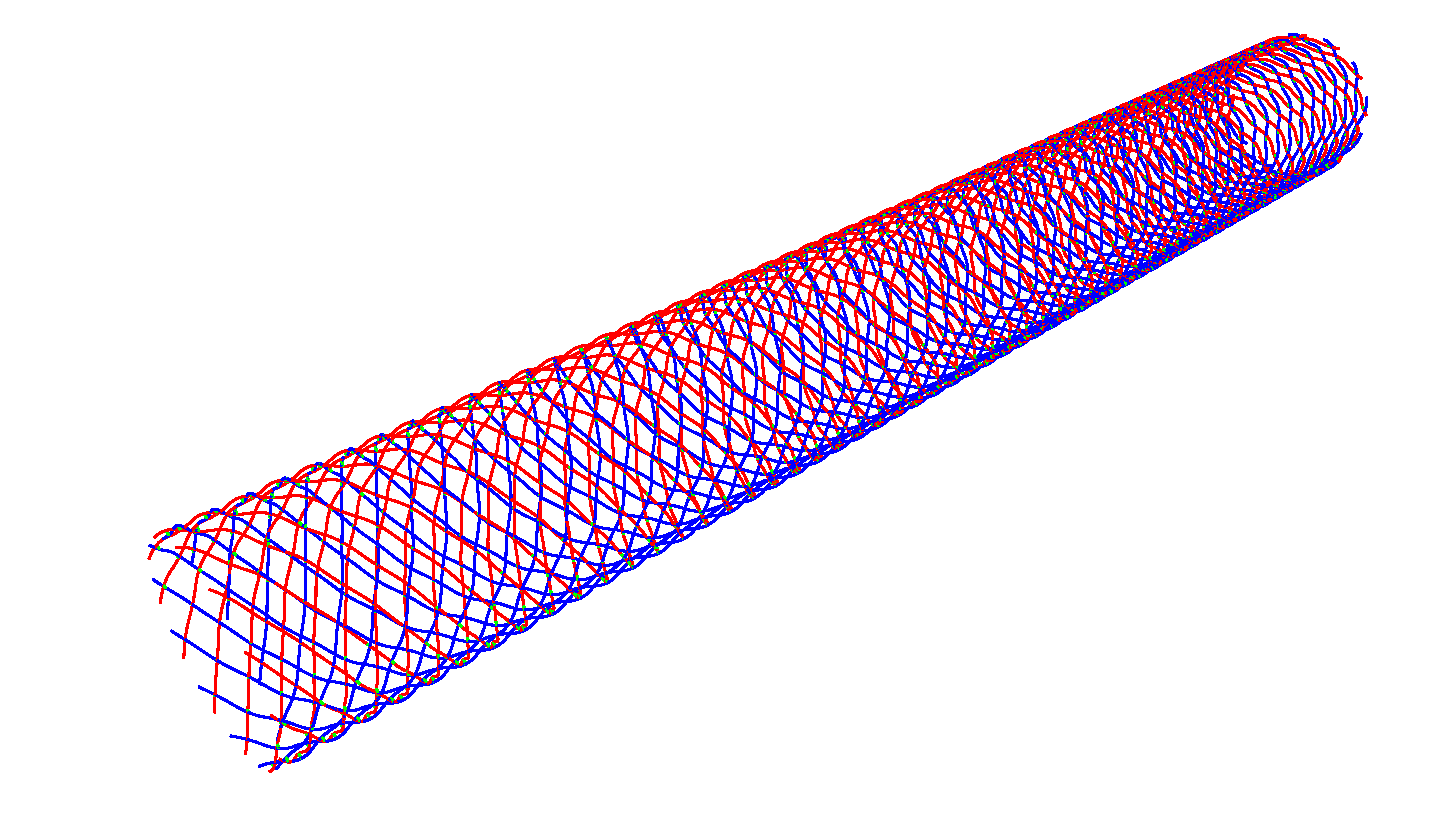
\includegraphics[width=12cm]{images/wirestent}
  \end{latexonly}
  \begin{htmlonly}
    \htmladdimg{../images/wirestent.png}
  \end{htmlonly}  
  \caption{WireStent example.}
\end{figure}

This structure is composed of 22032 line segments, each with 2 nodes. Nobody in his right mind would ever even try to input all the 132192 coordinates of all the points describing that structure. 
With \pyformex, one could define the structure by a sequence of operations like this:
 \begin{itemize}
 \item Create a planar base module of two crossing wires.
 \item Extend the base module with a mirrored and translated copy.
 \item Replicate the base module in both directions of the base plane.
 \item Roll the planar grid into a cylinder.
 \end{itemize}
 The procedure is illustrated by the subsequent images in the figure below.
 \begin{figure}[h]
   \centering
   \begin{makeimage}
   \end{makeimage}
   \begin{latexonly}
     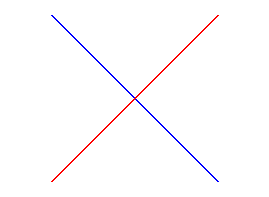
\includegraphics[width=2cm]{images/wirestent-1}
     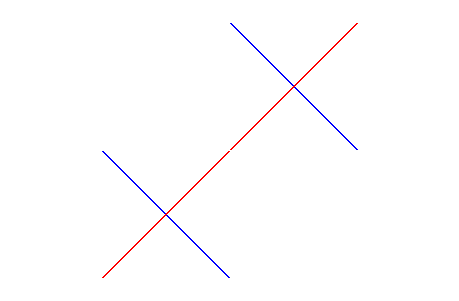
\includegraphics[width=2cm]{images/wirestent-2}
     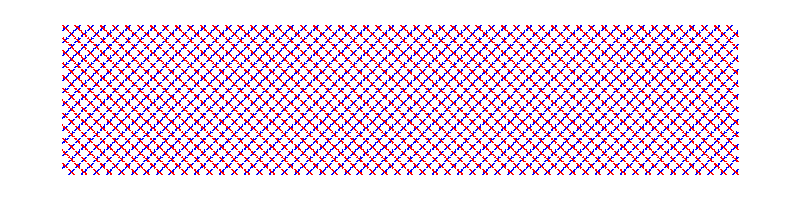
\includegraphics[width=12cm]{images/wirestent-3}
   \end{latexonly}
   \begin{htmlonly}
     \htmladdimg{../images/wirestent-1.png}
     \htmladdimg{../images/wirestent-2.png}
     \htmladdimg{../images/wirestent-3.png}
   \end{htmlonly}  
   \label{fig:WireStent steps}
   \caption{WireStent example.}
 \end{figure}


\section{Rationale}
\label{sec:rationale}
\pyformex does not fit into a single category of traditional (mostly commercial) software packages, because it is not being developed as a program with a specific purpose, but rather as a collection of tools we need is some of our research projects. Many of the tasks for which we now use \pyformex could as well or sometimes even better be done with some other software package, like a CAD program %(e.g. SolidWorks\textregistered)
or a %(MatLab\textregistered{} style)
matrix calculation package or a solid modeler/renderer %genre Blender
or a finite element preprocessor%(such as GiD)
. Each of these is very well suited for the task it was designed for, but none provides all the features of \pyformex in a single consistent packages. 

Perhaps the most important feature of \pyformex is that is was primarily intended to be an easy scripting language for creating geometrical models of 3D-structures. The Graphical User Interface was only added as a convenient means to visualize the designed structure. \pyformex can still run without user interface, and this makes it ideal for use in a batch toolchain.

The author of \pyformex, professor in structural engineering and heavy computer user since mainframe times, deeply regrets that computing skills of nowadays engineering students are often limited to using graphical interfaces of mostly commercial packages. This greatly limits their abilities, because in their mind: 'If there is no menu item to do a certain task, then it can not be done!'
The hope to get some of them back to coding has been a stimulus in continuing our work on \pyformex. 
 
Finally, \pyformex is, and will always be, free software in both meanings of free: guaranteeing your freedom (see \ref{sec:license}) and without paying. 


%\section{History}
%\label{sec:history}

\section{License and Disclaimer}
\label{sec:license}
\pyformex \copyright 2004-2007 Benedict Verhegghe

This program is free software; you can redistribute it and/or modify
it under the terms of the \htmladdnormallinkfoot{GNU General Public License}{http://www.gnu.org/licenses/gpl.html} as published by
the Free Software Foundation; either version 2 of the License, or
(at your option) any later version. 

Full details of the license are available in appendix \ref{cha:license} and in the file \textsf{COPYING} included with the distribution. 

This program is distributed in the hope that it will be useful,
but WITHOUT ANY WARRANTY; without even the implied warranty of
MERCHANTABILITY or FITNESS FOR A PARTICULAR PURPOSE.  See the
GNU General Public License for more details.


\section{Installation}
\label{sec:installation}
\subsection{Prerequisites}
\label{sec:prerequisites}
In order to run \pyformex, you need to have the following installed (and working) on your computer.
\begin{itemize}
\item \htmladdnormallinkfoot{Python}{\pythonURL}: Version 2.4 or higher is recommended. Versions 2.3 and 2.2 might work with only a few minor changes.
Nearly all Linux distributions come with Python installed, so this should not be no major obstacle.
\item \htmladdnormallinkfoot{NumPy}{\numpyURL}: Version 1.0-rc1 or higher. Earlier versions can be made to work, but will require some changes to be made. NumPy is the package we use for fast numerical array operations in Python and is essential for \pyformex.\footnote{The \texttt{Numarray} package, which was used up until \pyformex 0.3, is no longer supported }
On Linux systems, installing NumPy from source is usually straightforward. Debian users should install the packages python-numpy, python-numpy-dev and python-numpy-ext. There are binary packages for Windows on the \htmladdnormallinkfoot{Sourceforge download page}{http://www.numpy.org/}.
\end{itemize}
If you only want to use the Formex data model and transformation methods, this will suffice. But most probably you will also want to run the \pyformex Graphical User Interface (GUI) for visualizing your structures. Then you also need the following. 
\begin{itemize}
\item \htmladdnormallinkfoot{Qt4}{http://www.trolltech.com/products/qt}: The widget toolkit on which the GUI was built. For Debian users this  come in the packages python-qt4 and python-qt4-dev.
\item \htmladdnormallinkfoot{PyQt4}{http://www.riverbankcomputing.co.uk/pyqt/index.php}: The Python bindings for Qt4. Debian users shoould install the packages python-qt4, python-qt4-dev, python-qt4-gl.
\item \htmladdnormallinkfoot{PyOpenGL}{http://pyopengl.sourceforge.net/}: Pytong bindings for OpenGL, used for drawing and manipulating the 3D-structures. For denian users this is in package python-opengl.
\end{itemize}



\subsection{Downloading}
\label{sec:downloading}
The official releases of \pyformex can be downloaded from the 
\htmladdnormallinkfoot{\pyformex website}{\websiteURL}. As of the writing of this manual, the latest release is \htmladdnormallinkfoot{pyformex 0.4}{http://prdownload.berlios.de/pyformex/pyformex-0.4.tar.gz}. 
\pyformex is currently distributed in the form of a \Code{.tar.gz} (tarball) archive. See \ref{sec:installation-linux} for how to proceed further.

Alternatively you can download the tarball releases from our \htmladdnormallinkfoot{local FTP server}{ftp://bumps.ugent.be/pub/pyformex\xspace}. This one is slower, but you occasionally you might find there an interim release or release candidate not (yet) available on the official server.

Finally, you can also get the latest development code from the SVN repository on the \htmladdnormallinkfoot{\pyformex website}{\websiteURL}. If you have \htmladdnormallinkfoot{Subversion}{http://subversion.tigris.org/} installed on your system, you can just do\CodeLine{svn checkout svn://svn.berlios.de/pyformex/trunk \pyformex}
and the whole current \pyformex tree will be copied to a subdirectory \code{pyformex} on your current path.

\emph{Unless you absolutely need some of the latest features or bugfixes, the tarball releases are what you want to go for. 
}


\subsection{Installation on Linux platforms}
\label{sec:installation-linux}
Once you have downloaded the \pyformex tarball, unpack it with
\CodeLine{tar xvzf pyformex-version.tar.gz}
Then go to the created pyformex directory:
\CodeLine{cd pyformex-version}
and do
\CodeLine{make install}
This will install \pyformex in \Code{/usr/local/lib/pyformex-version}.
If you want to install somewhere else, you need to change the Makefile first.  

The installation procedure installs everything into this single directory, but also makes a couple of symlinks:
/usr/local/share/doc/pyformex-version is a link to the doc subdirectory of pyformex, ans /usr/local/bin/pyformex is a link to the main executable pyformex.py.


\subsection{Installation on Windows platforms}
\label{sec:installation-windows}
There is no installation procedure yet. All the pre-requisite packages are available for Windows, so in theory it is possible to run \pyformex on Windows. We know of some users who are running \pyformex succesfully using the --nogui option, i.e. without the Graphical User Interface (GUI).  
A few things may need to be changed for running the GUI on Windows. We will have a look at this in the future, but it is not our primary concern.
Still, any feedback on (succesful or not succesful) installation attempts on Windows is welcome.


\section{Running \pyf}
\label{sec:running}
To start \pyf, enter the command \Code{pyformex --gui}. This will start the \pyf Graphical User Interface (GUI), from where you can launch examples or load, edit and run your own \pyf scripts.

The installation procedure may have installed \pyf into your desktop menu or even have created a start button in the desktop panel. These provide convenient shortcuts to start the \pyf GUI.

The \pyf program takes some optional command line options, that modify the behaviour of the program.

\subsection{Command line options}
The whole list of possible command line options can be seen by executing the command \Code{pyformex --help}. This will produce the following output.
\verbatiminput{pyformex.help}

\emph{As of version 0.4.2, the\Code{--nogui} option has become the default. This is because the command line will mostly be used to start non-interactive execution of \pyf, while the GUI will often be launched from a start button or menu, which can easily incorporate the --gui option. 
}
\subsection{Running \pyFormex without the GUI}
If you start \pyf without the \Code{--gui} option, no Graphical User Interface is created. This is extremely useful to run automated scripts in batch mode. When run without the \Code{--gui} option, \pyf will interprete all arguments remaining after interpreting the options, as filenames of scripts to be run (and possibly arguments to be interpreted by these scripts).
Thus, if you want to run a \pyf script \Code{myscript.py} in batch mode, just give the command \Code{pyformex myscript.py}.
 

\section{Quick tutorial for the \pyformex GUI}
\label{sec:gui-tutorial}
In the current version () the GUI mainly serves the following purposes:
\begin{itemize}
\item Display a structure in 3D. This includes changing the viewpoint, orientation and viewing distance. Thus you can interactively rotate, translate, zoom.
\item Save a view in one of the supported image formats. Most of the images in this manual and on the \pyformex{} website were created that way. 
\item Changing \pyformex settings (though there aren't many yet that can be changed through the GUI).
\item Running \pyformex scripts, possibly starting other programs and display their results.
\item Interactively construct, change, import or export Formex structures. 
\end{itemize}

The GUI does not (yet) provide a means to interactively design a structure, select parts of a structure or set/show information about (parts of) the structure. Designing a structure is done by writing a small script with the mathematical expressions needed to generate it. Any text editor will be suitable for this purpose. The author uses XEmacs, but this is just a personal preference. 
A \pyformex editor integrated into the GUI remains on our TODO list, but it certainly is not our top priority, because general purpose editors are adequate for most of our purposes. 

Since \htmladdnormallinkfoot{Python}{\pythonURL} is the language used in \pyformex scripts, a Python aware editor is preferable. It will highlight the syntax and help you with proper alignment (which is very important in Python). 
 

The best way to learn to use \pyformex is by studying and changing some of the examples. I suggest that you first take a look at the examples included in the \pyformex GUI and select those that display structures that look interesting to you. Then you can study the source code of those examples and see how the structures got built. 
When starting up, \pyformex reads through the Examples directory (this is normally the 'examples' subdirecty located under the pyformex installation dir).  
\menuselection{Examples \sub WireStent}


\section{Quick {Python tutorial}}
\label{sec:python-tutorial}
\pyf is written in the Python language, and Python is also the scripting language of \pyf. Since the intent of \pyf is to design structures by using scripts, you will at least need to have some basic knowledge of Python before you can use \pyf for your own projects.

There is ample documentation about Python freely available on the \htmladdnormallinkfoot{web}{\pythonURL}. 
If you are new to Python, but have already some programming experience, the \htmladdnormallinkfoot{Python tutorial}{\pythonTUT} may be a good starting point.
Or else, you can take a look at one of the \htmladdnormallinkfoot{beginners' guides}{\pythonBEG}.


\section{Quick NumPy tutorial}
\label{sec:numpy-tutorial}
Numerical Python (or NumPy for short) is an extension to the Python language that allows for efficient operations on large (numerical) arrays. \pyf relies heavily on NumPy, and most likely you will need to use some NumPy functions in your scripts. As NumPy is still quite young, the available documentation is not so extensive yet. Still, the \htmladdnormallinkfoot{tentative NumPy tutorial}{http://www.scipy.org/Tentative_NumPy_Tutorial} already provides the basics.


%%% Local Variables: 
%%% mode: latex
%%% TeX-master: "manual"
%%% End: 
